\documentclass[border=10pt]{standalone} 
\usepackage{tikz}
\usetikzlibrary{calc, decorations.pathreplacing, arrows.meta} % Añadido arrows.meta
\usepackage{amsmath}
\usepackage{tkz-euclide}

\begin{document}
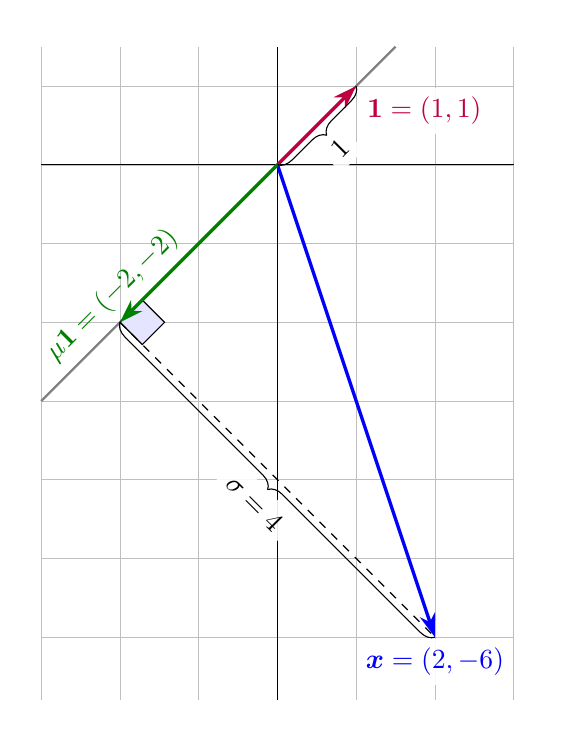
\begin{tikzpicture}
    % Establecer los límites del gráfico y agregar un grid
    \draw[step=1cm,lightgray,very thin] (-3,-6.8) grid (3,1.5);
    \draw[-, thin] (-3,0) -- (3,0) node[right]{};
    \draw[-, thin] (0,-6.8) -- (0,1.5) node[above]{};
    
    % Dibujar la recta generada por el vector (1,1)
    \coordinate (C1) at (-3,-3);
    \coordinate (C2) at ( 1.5, 1.5);
    \draw[-,thick,gray] (C1) -- (C2) node[right]{};

    % Definir los vectores
    \coordinate (O) at (0,0);
    \coordinate (U) at (1,1);
    \coordinate (X) at (2,-6);
    \coordinate (M) at ($(O)!(X)!(U)$);

    % Marca de ángulo recto
    \tkzMarkRightAngle[fill=blue!10,size=.4](O,M,X)

    % Dibujar el vector Uno
    \draw[-{Stealth[length=3mm, width=2mm]},very thick, purple] (O) -- (U) node[below right,fill=white,opacity=.9,text opacity=1]{$\boldsymbol{1}=(1,1)$};
    
    % Dibujar el vector X
    \draw[-{Stealth[length=3mm, width=2mm]},very thick, blue] (O) -- (X) node[below, sloped,fill=white,opacity=.9,text opacity=1]{$\boldsymbol{x}=(2,-6)$};
    
    % Dibujar el vector (-2,-2)
    %\node[green!50!black,align=center,fill=white,opacity=.9,text opacity=1] at (M) {$\mu\boldsymbol{1}=(-2,-2)$};
    \draw[-{Stealth[length=3mm, width=2mm]},very thick,green!50!black] (O) -- (M) node[midway, above left, sloped,text opacity=1]{$\mu\boldsymbol{1}=(-2,-2)$};
    
    % Dibujar la línea punteada entre (-2,-2) y (2,-6)
    \draw[dashed] (M) -- (X);
    
    % Añadir una llave con la etiqueta sigma
    \draw[decorate,decoration={brace,amplitude=5pt,mirror},xshift=0pt,yshift=0pt] (M) -- (X) node[midway, below,  yshift=-5pt, sloped,fill=white,opacity=.9,text opacity=1] {$\sigma=4$};

    % Añadir una llave con longitud del vector uno
    \draw[decorate,decoration={brace,amplitude=5pt,mirror},xshift=0pt,yshift=0pt] (O) -- (U) node[midway, below,  yshift=-5pt, sloped,fill=white,opacity=.9,text opacity=1] {$1$};

\end{tikzpicture}
\end{document}
